\subsection{x86}

\subsubsection{\NonOptimizing MSVC}

\RU{Это дает в итоге}\EN{Result} (MSVC 2010):

\lstinputlisting[caption=MSVC 2010]{patterns/08_switch/1_few/few_msvc.asm}

\RU{Наша функция со оператором switch(), с небольшим количеством вариантов, 
это практически аналог подобной конструкции:}
\EN{Our function with a few cases in switch() is in fact analogous to this construction:}

\lstinputlisting[label=switch_few_ifelse]{patterns/08_switch/1_few/few_analogue.c}

\index{\CLanguageElements!switch}
\index{\CLanguageElements!if}
\RU{Когда вариантов немного и мы видим подобный код, невозможно сказать с уверенностью, был ли
в оригинальном исходном коде switch(), либо просто набор операторов if().}
\EN{If we work with switch() with a few cases it is impossible to be sure if it was
a real switch() in the source code, or just a pack of if() statements.}
\index{\SyntacticSugar}
\RU{То есть, switch() это синтаксический сахар для большого количества вложенных проверок 
при помощи if().}
\EN{This implies that switch() is like syntactic sugar for a large number of nested if()s.}

\RU{В самом выходном коде ничего особо нового, 
за исключением того, что компилятор зачем-то 
перекладывает входящую переменную ($a$) во временную в локальном стеке \TT{v64}%
\footnote{Локальные переменные в стеке с префиксом \TT{tv}~--- 
так MSVC называет внутренние переменные для своих нужд}.}
\EN{There is nothing especially new to us in the generated code,
with the exception of the compiler moving 
input variable 
$a$ to a temporary local variable \TT{tv64}
\footnote{Local variables in stack are prefixed with \TT{tv}---%
that's how MSVC names internal variables for its needs}.}

\RU{Если скомпилировать это при помощи GCC 4.4.1, то будет почти то же самое, даже с максимальной оптимизацией 
(ключ \Othree).}
\EN{If we compile this in GCC 4.4.1, we'll get almost the same result, even with maximal optimization
turned on (\Othree option).}

\subsubsection{\Optimizing MSVC}

\RU{Попробуем включить оптимизацию кодегенератора}%
% TODO separate various kinds of \TT
% idea: enclose command lines in a specific environment, like \cmdline{} 
% assembly instructions in \asm{} (now both \TT and \q{} are used),
% variables in,  like \var{}
% messages (string constants) in something else, like \strconst
% to separate them all. Now they all use \TT, which is not best
% \INS{} for all instructions including operands? --DY
\EN{Now let's turn on optimization in} MSVC (\Ox): \TT{cl 1.c /Fa1.asm /Ox}

\label{JMP_instead_of_RET}
\lstinputlisting[caption=MSVC]{patterns/08_switch/1_few/few_msvc_Ox.asm}

\RU{Вот здесь уже всё немного по-другому, причем не без грязных трюков.}
\EN{Here we can see some dirty hacks.}

\index{x86!\Instructions!JZ}
\index{x86!\Instructions!JE}
\index{x86!\Instructions!SUB}
\RU{Первое: \TT{а} помещается в \EAX и от него отнимается 0. Звучит абсурдно, но нужно это для того, чтобы проверить, 
0 ли в \EAX был до этого? Если да, то выставится флаг \ZF (что означает, что результат вычитания 0 от числа 
стал 0) и первый условный переход \JE (\IT{Jump if Equal} или его синоним \JZ~--- \IT{Jump if Zero}) 
сработает на метку \TT{\$LN4@f}, где выводится сообщение \TT{'zero'}.
Если первый переход не сработал, от значения отнимается по единице, 
и если на какой-то стадии в результате образуется 0, то сработает соответствующий переход.}
\EN{First: the value of $a$ is placed in \EAX and 0 is subtracted from it. Sounds absurd, but it is done to check if 
the value in \EAX was 0. If yes, the \ZF flag is to be set (e.g. subtracting from 0 is 0) 
and the first conditional jump \JE (\IT{Jump if Equal} or synonym \JZ~---\IT{Jump if Zero}) is to be triggered 
and control flow is to be passed to the \TT{\$LN4@f} label, where the \TT{'zero'} message is being printed. 
If the first jump doesn't get triggered, 1 is subtracted from the input value and if at some stage the result is 0, 
the corresponding jump is to be triggered.}

\RU{И в конце концов, если ни один из условных переходов не сработал, управление передается \printf
со строковым аргументом \TT{'something unknown'}.}
\EN{And if no jump gets triggered at all, the control flow passes to \printf with string argument \TT{'something unknown'}.}

\label{jump_to_last_printf}
\index{\Stack}
\RU{Второе: мы видим две, мягко говоря, необычные вещи: указатель на сообщение помещается в переменную $a$, 
и затем \printf вызывается не через \CALL, а через \JMP. Объяснение этому простое. 
Вызывающая функция заталкивает в стек некоторое значение и через \CALL вызывает нашу функцию. 
\CALL в свою очередь заталкивает в стек адрес возврата (\ac{RA}) и делает безусловный переход на адрес нашей функции. 
Наша функция в самом начале (да и в любом её месте, потому что в теле функции нет ни одной инструкции, 
которая меняет что-то в стеке или в \ESP) имеет следующую разметку стека:}
\EN{Second: we see something unusual for us: a string pointer is placed into the $a$ variable, and 
then \printf is called not via \CALL, but via \JMP. There is a simple explanation for that: 
the \gls{caller} pushes a value to the stack and calls our function via \CALL. 
\CALL itself pushes the return address (\ac{RA}) to the stack and does an unconditional jump to our function address. 
Our function at any point of execution (since it do not contain any instruction that moves the stack 
pointer) has the following stack layout:}

\begin{itemize}
\item\ESP\EMDASH\RU{хранится}\EN{points to} \ac{RA}
\item\TT{ESP+4}\EMDASH\RU{хранится значение $a$}\EN{points to the $a$ variable} 
\end{itemize}

\RU{С другой стороны, чтобы вызвать \printf, нам нужна почти такая же разметка стека, 
только в первом аргументе нужен указатель на строку. Что, собственно, этот код и делает.}
\EN{On the other side, when we need to call \printf here we need exactly the same stack 
layout, except for the first \printf argument, which needs to point to the string. 
And that is what our code does.}

\RU{Он заменяет свой первый аргумент на адрес строки, и затем передает управление \printf, как если бы вызвали не 
нашу функцию \ttf, а сразу \printf. 
\printf выводит некую строку на \gls{stdout}, затем исполняет инструкцию \RET, 
которая из стека достает \ac{RA} и управление передается в ту функцию, 
которая вызывала \ttf, минуя при этом конец функции \ttf.}
\EN{It replaces the function's first argument with the address of the string and 
jumps to \printf, as if we didn't call our function \ttf, but directly \printf.
\printf prints a string to \gls{stdout} and then executes the \RET instruction, which POPs 
\ac{RA} from the stack and control flow is returned not to \ttf but rather to \ttf's \gls{callee}, 
bypassing the end of the \ttf function.}

\index{\CStandardLibrary!longjmp()}
\newcommand{\URLSJ}{\href{http://go.yurichev.com/17121}{wikipedia}}
\RU{Всё это возможно, потому что \printf вызывается в \ttf в самом конце. 
Всё это чем-то даже похоже на \TT{longjmp()}\footnote{\URLSJ}.
И всё это, разумеется, сделано для экономии времени исполнения.}
\EN{All this is possible because \printf is called right at the end of the \ttf function in all cases. 
In some way, it is similar to the \TT{longjmp()}\footnote{\URLSJ} function.
And of course, it is all done for the sake of speed.}

\ifdefined\IncludeARM
\RU{Похожая ситуация с компилятором для ARM описана в секции}
\EN{A similar case with the ARM compiler is described in} \q{\PrintfSeveralArgumentsSectionName}%
\EN{section, here}~(\myref{ARM_B_to_printf}).
\fi

\ifdefined\IncludeOlly
\clearpage
\myparagraph{\olly}

\RU{Так как этот пример немного запутанный, попробуем оттрассировать его в}\EN{Since this example is tricky, 
let's trace it in} \olly.\\
\\
\olly \RU{может распознавать подобные switch()-конструкции, так что он добавляет полезные комментарии}\EN{can 
detect such switch() constructs, and it can add some useful comments}.
\EAX \RU{в начале равен}\EN{is} 2\EN{ in the beginning}, \RU{это входное значение функции}\EN{that's the function's input value}: 

\begin{figure}[H]
\centering
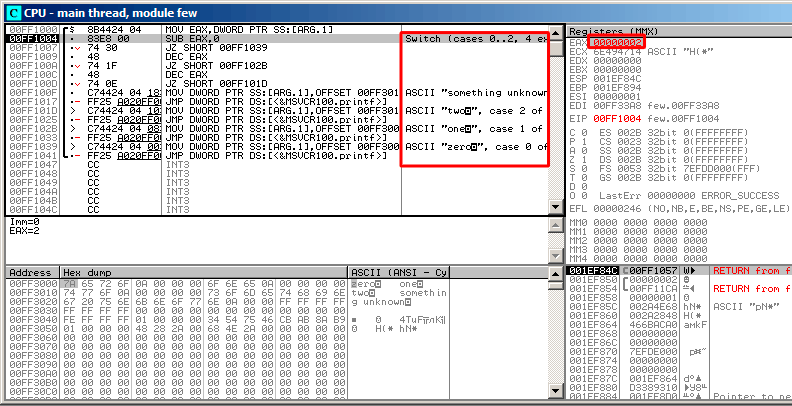
\includegraphics[scale=\FigScale]{patterns/08_switch/1_few/olly1.png}
\caption{\olly: \EAX \RU{содержит первый (и единственный) аргумент функции}
\EN{now contain the first (and only) function argument}}
\label{fig:switch_few_olly1}
\end{figure}

\clearpage
0 \RU{отнимается от}\EN{is subtracted from} 2 \InENRU \EAX. 
\RU{Конечно же}\EN{Of course}, \EAX \RU{всё ещё содержит}\EN{still contains} 2.
\RU{Но флаг}\EN{But the} \ZF \RU{теперь}\EN{flag is now} 0, \RU{что означает, что последнее вычисленное значение
не было нулевым}\EN{indicating that the resulting value is non-zero}:

\begin{figure}[H]
\centering
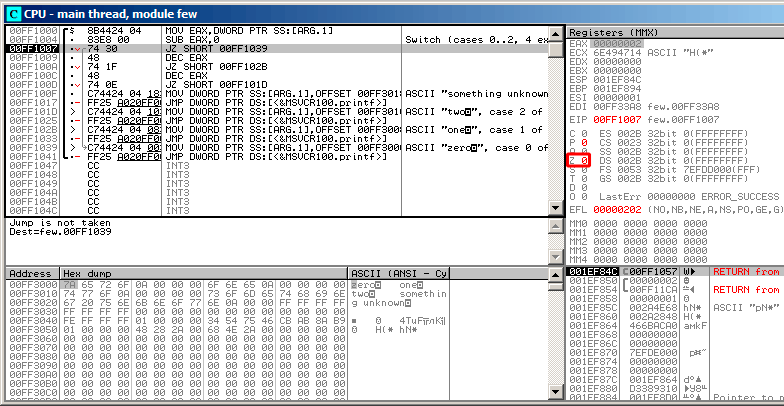
\includegraphics[scale=\FigScale]{patterns/08_switch/1_few/olly2.png}
\caption{\olly: \SUB \RU{исполнилась}\EN{executed}}
\label{fig:switch_few_olly2}
\end{figure}

\clearpage
\DEC \RU{исполнилась и}\EN{is executed and} \EAX \RU{теперь содержит}\EN{now contains} 1. 
\RU{Но}\EN{But} 1 \RU{не ноль, так что флаг}\EN{is non-zero, so the} \ZF \RU{всё ещё}\EN{flag is still} 0:

\begin{figure}[H]
\centering
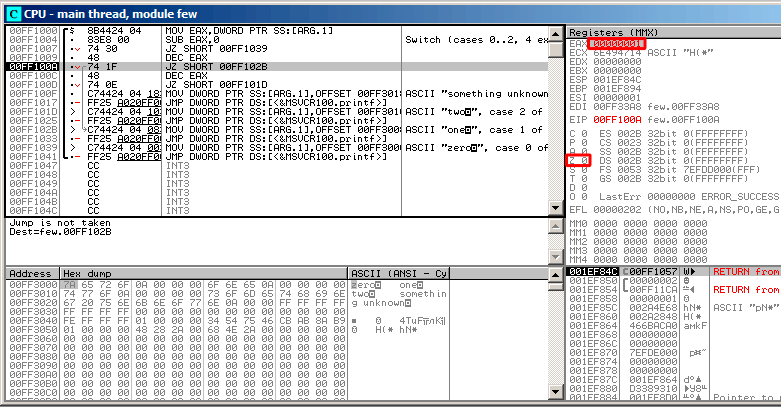
\includegraphics[scale=\FigScale]{patterns/08_switch/1_few/olly3.png}
\caption{\olly: \RU{первая}\EN{first} \DEC \RU{исполнилась}\EN{executed}}
\label{fig:switch_few_olly3}
\end{figure}

\clearpage
\RU{Следующая}\EN{Next} \DEC \RU{исполнилась}\EN{is executed}. 
\EAX \RU{наконец}\EN{is finally} 0 \RU{и флаг}\EN{and the} \ZF \RU{выставлен, потому что результат~--- ноль}\EN{flag
gets set, because the result is zero}:

\begin{figure}[H]
\centering
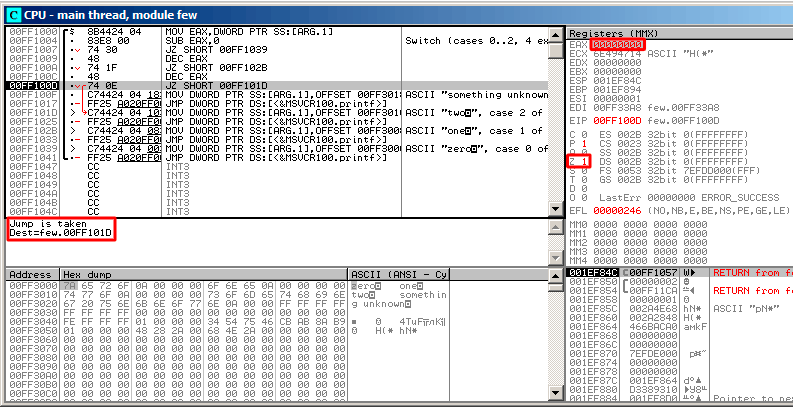
\includegraphics[scale=\FigScale]{patterns/08_switch/1_few/olly4.png}
\caption{\olly: \RU{вторая}\EN{second} \DEC \RU{исполнилась}\EN{executed}}
\label{fig:switch_few_olly4}
\end{figure}

\olly \RU{показывает, что условный переход сейчас сработает.}
\EN{shows that this jump is to be taken now.}

\clearpage
\RU{Указатель на строку}\EN{A pointer to the string} \q{two} 
\RU{сейчас будет записан в стек}%
\EN{is to be written into the stack now}:

\begin{figure}[H]
\centering
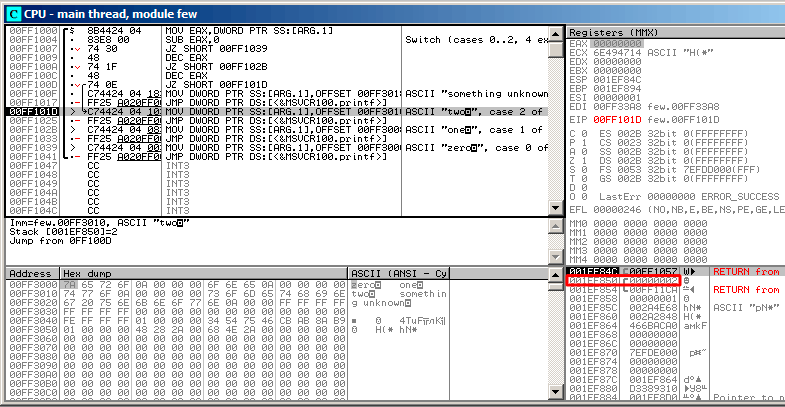
\includegraphics[scale=\FigScale]{patterns/08_switch/1_few/olly5.png}
\caption{\olly: \RU{указатель на строку сейчас запишется на место первого аргумента}
\EN{pointer to the string is to be written at the place of the first argument}}
\label{fig:switch_few_olly5}
\end{figure}

% TODO: homogenize numbers
% now they are inconsistent: sometimes plain text, sometimes in math mode
% some kind of \expr{} both for numbers and expressions? --DY
\RU{Обратите внимание: текущий аргумент функции это 2 и 2 прямо сейчас в стеке по адресу}\EN{Please note: 
the current argument of the function is 2 and 2 is now in the stack at the address} \TT{0x001EF850}.

\clearpage
\MOV \RU{записывает указатель на строку по адресу}\EN{writes the pointer to the string at address} 
\TT{0x001EF850} (\RU{см. окно стека}\EN{see the stack window}).
\RU{Переход сработал}\EN{Then, jump happens}.
\RU{Это самая первая инструкция функции}\EN{This is the first instruction of the} \printf \RU{в}\EN{function in} 
MSVCR100.DLL (\RU{этот пример был скомпилирован с опцией /MD}\EN{This example was compiled with /MD switch}): 

\begin{figure}[H]
\centering
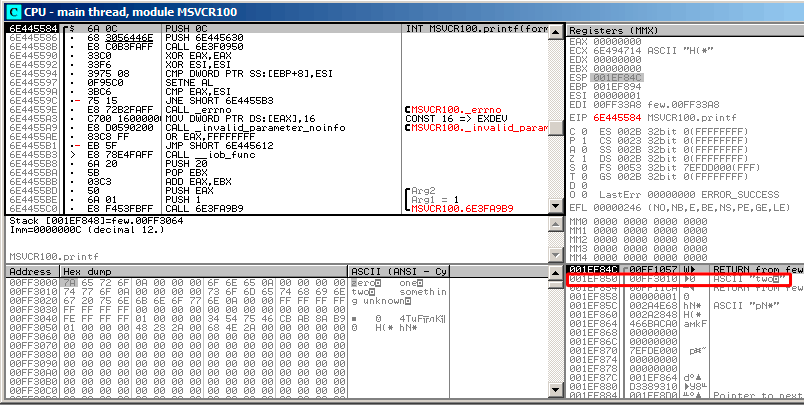
\includegraphics[scale=\FigScale]{patterns/08_switch/1_few/olly6.png}
\caption{\olly: \RU{первая инструкция в}\EN{first instruction of} \printf \InENRU MSVCR100.DLL}
\label{fig:switch_few_olly6}
\end{figure}

\RU{Теперь}\EN{Now} \printf \RU{считает строку на}\EN{treats the string at} \TT{0x00FF3010} 
\RU{как свой единственный аргумент и выводит строку}\EN{as its only argument and prints the string}.

\clearpage
\RU{Это самая последняя инструкция функции}\EN{This is the last instruction of} \printf:

\begin{figure}[H]
\centering
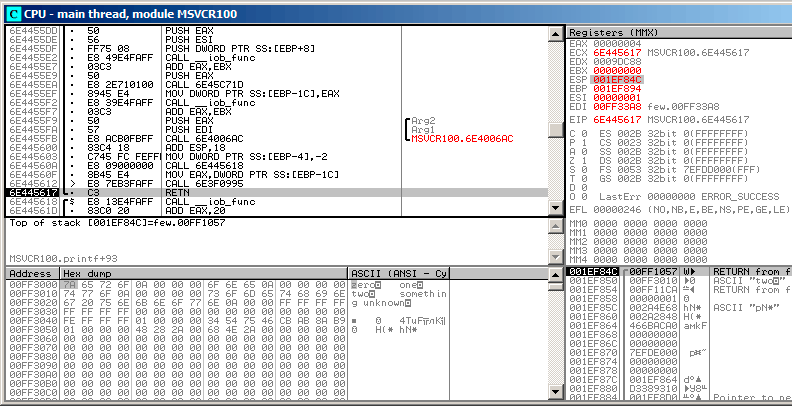
\includegraphics[scale=\FigScale]{patterns/08_switch/1_few/olly7.png}
\caption{\olly: \RU{последняя инструкция в}\EN{last instruction of} \printf \InENRU MSVCR100.DLL}
\label{fig:switch_few_olly7}
\end{figure}

\EN{The string}\RU{Строка} \q{two} \RU{была только что выведена в консоли}\EN{was just printed to the console window}.

\clearpage
\RU{Нажмем}\EN{Now let's press} F7 \OrENRU F8 (\stepover) \RU{и вернемся}\EN{and return}\dots
\RU{нет, не в функцию}\EN{not to} \ttf \RU{но в}\EN{, but rather to} \main:

\begin{figure}[H]
\centering
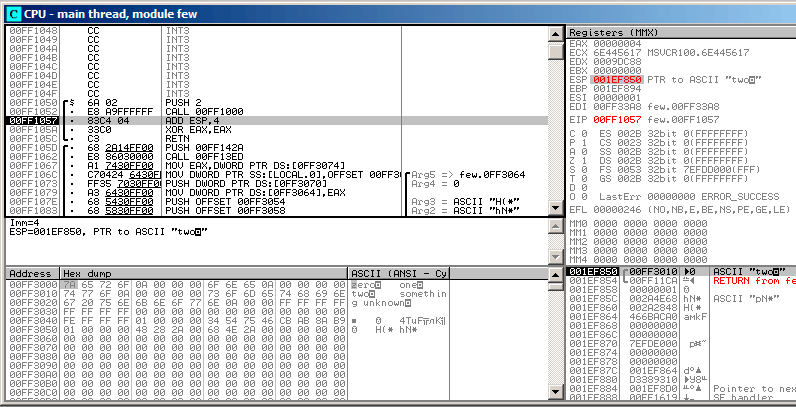
\includegraphics[scale=\FigScale]{patterns/08_switch/1_few/olly8.png}
\caption{\olly: \RU{возврат в}\EN{return to} \main}
\label{fig:switch_few_olly8}
\end{figure}

\RU{Да, это прямой переход из внутренностей}\EN{Yes, the jump was direct, from the guts of} \printf 
\RU{в}\EN{to} \main.
\RU{Потому как}\EN{Because} \ac{RA} \RU{в стеке указывает не на какое-то место в функции}\EN{in the stack points 
not to some place in} \ttf \RU{а в}\EN{, but rather to} \main.
\RU{И}\EN{And} \CALL \TT{0x00FF1000} \RU{это инструкция вызывающая функцию}\EN{was the actual instruction which called} 
\ttf.

\fi
